\chapter{The Quest for Meaning in Video}
\label{ch:quest}

\section{Introduction} % (fold)
\label{sec:introduction}

% start intro: consider example of a video segment; indicate how its easy for humans to `understand' the content on multiple levels
Interpreting moving images is not a hard task. The medium film is often described as `dictatorial' because of the way the audience is immersed in a multi-modal experience controlled by the creators. We can sit back and relax, passively taking in the presented information without much effort. A similar ease is reflected in our use of the word `couch potato' to describe the passive role of television audiences. Watching film or video gives us almost immediate access to a wide range of information about what is presented on screen. We recognise objects on screen and understand words that spoken in a language we know. We are also quick to infer a larger picture around the things we perceive, like personality traits of characters on screen or our emotional stance towards them. While most of these things happen extremely quickly and seemingly automatically to us humans, computers often have a hard time even starting to perceive a visual representation of an object.

% explain how computers are having difficulties. in recognition, spatio/temporal segmentation (figure ground), qualitative evaluations are even more difficult.
When we attend to visual content depicting parts of the world around us, we can't help ourselves from seeing its parts as separate entities. We recognise objects as if they stand out from their background even though they are simply patterns of colours on a two dimensional surface. To a computer, tasks like object segmentation and recognition are hard because visual information needs to be interpreted in some form of sequential processing. Digitally, images are usually represented by collections of numbers indicating local intensities (e.g. brightness) at the different points that make up the image. How to calculate from this information, which objects are present, and what other concepts can be assigned to an image is studied in the field of computer vision. Although recent years have seen important advances in the use of high-level semantical concepts in tasks like video concept detection and concept-based video retrieval \cite{Snoek:2009dq, Snoek:jf, Worring:2007vm, Chang:2008wh}, computational methods commonly have difficulties in performing both reliably and generally.

% from world -> representation -> concepts
To better understand what is going on in the interpretation of visual content by both humans and computers, it helps to model it as a process from start to end. Figure \ref{fig:understanding_visuals} shows in a high-level model how objects in the world are sensed and consequently rendered in a visual representation. We can think of this process taking place when we photograph a car and end up with a picture of that car as a result. When the representation of an object is next interpreted by someone, we can think of this person as establishing semantical concepts relating to aspects of the depiction. A situation to which we can map this part of the model would be someone looking at the picture and recognising the car.

\begin{figure}[htbp]
  \centering
    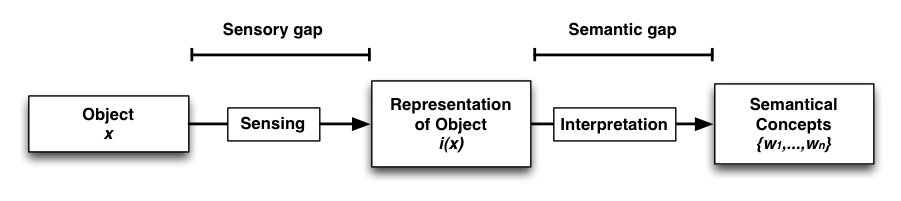
\includegraphics[width=.8\textwidth]{img/understanding_visuals}
  \caption{A high level model of the interpretation of visual media content}
  \label{fig:understanding_visuals}
\end{figure}

% first problem: sensory gap
A first source of complication in the process from object to its interpretation, is the \emph{sensory gap}, described by Smeulders et al. as follows:

\begin{quote}
  ``The sensory gap is the gap between the object in the world and the information in a (computational) description derived from a recording of that scene.''\cite{Smeulders:2000tx}
\end{quote}

% sensory gap explained
The sensory gap makes accurate description of objects in the world difficult as it introduces uncertainty about what aspects of the object are represented. Characteristics of illumination, occlusion, clutter and camera viewpoint all affect the representation of a sensed object. When detailed knowledge about the recording conditions is absent, it is impossible to know which parts of the sensory information should be attributed to the state of the object and which are due to incidental artefacts. Different 3D objects can yield the same 2D representation and differently coloured objects might be represented by identical colour values. This also works the other way, as one object may appear very different in shape and colour on different images depending on illumination and camera viewpoint.

% second problem: semantic gap
A second issue that hampers meaningful interpretation of visual content is the \emph{semantic gap} that lies between a digital representation and the conceptual interpretation we address to it. Snoek and Worring adapt the original definition from \cite{Smeulders:2000tx} to specifically fit the medium video when they describe the semantic gap as:

\begin{quote}
  ``The lack of correspondence between the low-level features that machines extract from video and the high-level conceptual interpretations a human gives to the data in a given situation.''
\end{quote}

One of the causes of the semantic gap is that the way people perceive images is mostly contextual\cite{Smeulders:2000tx}. We look for concepts that are already familiar from our environment or earlier encounters with visual content. Our perception of a simple object is determined by our vast background of personal experience and cultural upbringing. I might for example interpret a picture of a unicycle very different from someone who has never seen one before.

% subjecting interpretations; feeling and emotions
Another cause of the gap are interpretations that are subjective in nature. Semantical concepts relating to feelings and emotions can vary widely across different people. Deciding computationally whether concepts such as ``romantic'' or ``funny'' apply to a piece of content is hard when there is no agreement about the interpretation to begin with.

Concepts we perceive are also combined to infer a larger story around the things we actually see. These knowledge-based interpretations enable us to perceive deeper layers of meaning that are not in itself explicitly represented. An important example of this is the way `readers' of narrative texts or moving images combine elements in their aim for \emph{coherence}\cite[p.~38]{Bordwell:1985tz} \cite{gernsbacher1995coherence, Graesser:1994va}. 

In contrast to these contextual interpretations, computational image descriptions rely purely on data-driven features that can be extracted from the content. Difficulties arise when there is a mismatch between the two.

large variety in appearance of visual concepts
e.g. windmill
% symbolic, sensory

% scope of this chapter
Because of the often elusive character of concepts like meaning and understanding, we take care to keep our intentions for this chapter humble. The intension is not to give an accurate explanation of daunting concepts like meaning or semantics, nor is it to give an accurate account of the diverse work on the relationship between signifier and signified in the field of semiotics. This first chapter is meant to briefly introduce the difficulties that current computational methods have in arriving at a meaningful interpretation of visual content. To this purpose we formulate a framework of computational analyses of meaning that serves to establish terminology to work with in the remainder of this work, rather than to make claims about the deeper functioning of human understanding or signifying systems.



% section introduction (end)

\section{Computational Undertakings of the Quest for Meaning}

\subsection{Meaning in Visuals}
[Video structuring, indexing and retrieval based on global motion wavelet coefficients]\cite{Bruno:2002tt}

\subsection{Meaning in Concept}
\subsection{Meaning in Structure}
[cite bordwell \& Thompson: analysis of context dependency]
% hypervideo as form of 1 narrative 2 navigation, link to database documentary
[HyperCafe: Narrative and Aesthetic Properties of Hypervideo \cite{Sawhney:1996tk}]

\subsection{Meaning in Annotations}
[Telop-on-demand: Video structuring and retrieval based on text recognition]\cite{Kuwano:2000wy}
[Addressing the Challenge of Visual Information Access from Digital Image and Video Libraries]\cite{Christel:2005td}

\section{Computational Undertakings of the Quest}
\subsection{The Semantic Gap}


\subsection{Steps towards Meaning: An Overview}
Schematized summary of different steps:
indexing
automatic metadata
annotating
  Human-Driven Labeling
  Machine-Driven Labeling
multimodal feature fusion
concept based
content based [Relevance feedback: A power tool for interactive content-based image retrieval]\cite{Rui:1998uj}
[The Relative Effectiveness of Concept-based Versus Content-based Video Retrieval]\cite{Yang:2004tc}

[collaborative filtering] \url{http://en.wikipedia.org/wiki/Collaborative_filtering}

\subsection{Indexing to enable search}
Because visual data on it's own provides little machine-readable handles to search and find, repositories of multimedia content need to be index to enable search. Within the task of video indexing several approaches are taken 

\section{Computational Difficulties}

% problem is that no CV algorithms perform reliable AND generally

% the problem of acquiring labelled data for ML approaches
% problem of keeping ML techniques up to date in a dynamical environment where new content is added every minute (and a lot of it as we will see when we discuss user generated online video)





